\documentclass{beamer}
\usepackage{amsmath,amsbsy,amsopn,amstext,amsfonts,amssymb}
\usepackage{isomath}
\usepackage{ulem}
%\linespread{1.6}  % double spaces lines
\usepackage{graphicx}
\usepackage{subfigure}
\usepackage{color}
\usepackage{optidef}  % define optimization problems
\usepackage{multicol}  % multiple columns
\usepackage{listings} % for python code
\usepackage{mathrsfs}

\usepackage{polynom}
\newcommand{\adj}{\mathrm{adj}}
\newcommand{\constrainedmin}[3]{
		\begin{mini*}|s|
		{#2}{#1}{}{}
		\addConstraint{#3}
		\end{mini*}
}

\newcommand{\rwbcomment}[1]{{\color{blue}RWB:#1}}
\newcommand{\defeq}{\stackrel{\triangle}{=}}
\newcommand{\abs}[1]{\left|#1\right|}
\newcommand{\norm}[1]{\left\|#1\right\|}
\newcommand{\iprod}[1]{\left<#1\right>}
\newcommand{\ellbf}{\boldsymbol{\ell}}
\newcommand{\nubf}{\boldsymbol{\nu}}
\newcommand{\mubf}{\boldsymbol{\mu}}
\newcommand{\abf}{\mathbf{a}}
\newcommand{\bbf}{\mathbf{b}}
\newcommand{\cbf}{\mathbf{c}}
\newcommand{\dbf}{\mathbf{d}}
\newcommand{\ebf}{\mathbf{e}}
\newcommand{\fbf}{\mathbf{f}}
\newcommand{\gbf}{\mathbf{g}}
\newcommand{\hbf}{\mathbf{h}}
\newcommand{\ibf}{\mathbf{i}}
\newcommand{\jbf}{\mathbf{j}}
\newcommand{\kbf}{\mathbf{k}}
\newcommand{\lbf}{\mathbf{l}}
\newcommand{\mbf}{\mathbf{m}}
\newcommand{\nbf}{\mathbf{n}}
\newcommand{\obf}{\mathbf{o}}
\newcommand{\pbf}{\mathbf{p}}
\newcommand{\qbf}{\mathbf{q}}
\newcommand{\rbf}{\mathbf{r}}
\newcommand{\sbf}{\mathbf{s}}
\newcommand{\tbf}{\mathbf{t}}
\newcommand{\ubf}{\mathbf{u}}
\newcommand{\vbf}{\mathbf{v}}
\newcommand{\wbf}{\mathbf{w}}
\newcommand{\xbf}{\mathbf{x}}
\newcommand{\ybf}{\mathbf{y}}
\newcommand{\zbf}{\mathbf{z}}
\newcommand{\Jbf}{\mathbf{J}}
\newcommand{\Acal}{\mathcal{A}}
\newcommand{\Bcal}{\mathcal{B}}
\newcommand{\Lcal}{\mathcal{L}}
\newcommand{\Ncal}{\mathcal{N}}
\newcommand{\Rcal}{\mathcal{R}}
\definecolor{darkolivegreen}{rgb}{0.33, 0.42, 0.18}

\makeatletter
\newenvironment<>{proofstart}[1][\proofname]{%
    \par
    \def\insertproofname{#1\@addpunct{.}}%
    \usebeamertemplate{proof begin}#2}
  {\usebeamertemplate{proof end}}
\newenvironment<>{proofcont}{%
  \setbeamertemplate{proof begin}{\begin{block}{}}
    \par
    \usebeamertemplate{proof begin}}
  {\usebeamertemplate{proof end}}
\newenvironment<>{proofend}{%
    \par
    \pushQED{\qed}
    \setbeamertemplate{proof begin}{\begin{block}{}}
    \usebeamertemplate{proof begin}}
  {\popQED\usebeamertemplate{proof end}}
\makeatother

\title{ECEn 671: Mathematics of Signals and Systems}
\author{Randal W. Beard}
\institute{Brigham Young University}
\date{\today}

\begin{document}

%-------------------------------
\begin{frame}
	\titlepage
\end{frame}



%%%%%%%%%%%%%%%%%%%%%%%%%%%%%%%%%%%%%%%%%%%%%%%%%%%%%%%%%%%%%%%%%%%%%%%
\section{Projections}
\frame{\sectionpage}

%----------------------------------
\begin{frame}\frametitle{Projections}
\begin{itemize}
%\item This topic is probably the most important and useful topic covered in
%this class.  We will use it over and over.

\item Suppose that $V$ and $W$ are disjoint subspaces of $S$ such that $V + W = S$, i.e.
\[ x \in S \Rightarrow x = v + w\]
where $v \in V$ and $w \in W$ is a unique decomposition.

\item Define the linear operator $P:S\to V \subset S$ as 
\[ Px = P(v+w) = v \]

\item Note that $P(Px) = Pv = v$
\end{itemize}
	
\end{frame}

%----------------------------------
\begin{frame}\frametitle{Projections, cont.}
\begin{definition}[Projection Operator] 
Let $P: S \to S$ such that $P^2 = P$,
then $P$ is called a \underline{projection} operator or \underline{idempotent}.	
\end{definition}

\begin{example}
Let $P = \left( \begin{array}{cc} 1 & 0
    \\ 0 & 0 \end{array} \right)$, then $P\left( \begin{array}{c} x_1
    \\ x_2 \end{array} \right) = \left( \begin{array}{c} x_1 \\
    0 \end{array} \right)$\\
i.e. $P$ projects elements of $P$ onto the $x_1$ axis:

\begin{center}
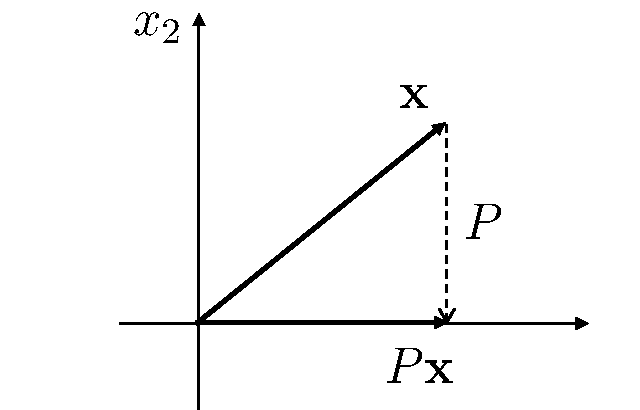
\includegraphics[width=2in]{figures/chap2_projection_1}
\end{center}

\end{example}
\end{frame}

%----------------------------------
\begin{frame}\frametitle{Projections, cont.}
\begin{example}
Truncation: let 
\[
(P_T x)(t) = \begin{cases} x(t), &\quad -T \leq t \leq T\\
0, &\quad \text{ otherwise }\end{cases}
\]
Then $P_T$ projects $x(t)$ onto its truncated function:\\

\begin{center}
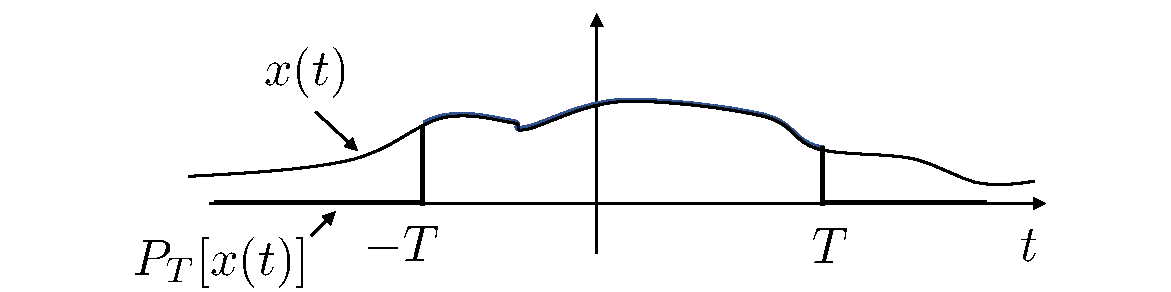
\includegraphics[width=4in]{figures/chap2_projection_2}	
\end{center}
\end{example}
\end{frame}

%----------------------------------
\begin{frame}\frametitle{Projections, cont.}
\begin{theorem}[Moon 2.7]
Let $P:S\to S$ be a projection operator, then
\[ 
S = R(P) + N(P) 
\]	
\end{theorem}
\begin{proof}
Homework problem.	
\end{proof}
\end{frame}

%----------------------------------
\begin{frame}\frametitle{Projections, cont.}
\begin{theorem}
	If $P:S\to S$ is a projection operator then so is $(I - P):S\to S$
\end{theorem}
\begin{proof}
\begin{flalign*}
  (I - P)^2 &= (I - P)(I - P) = \\
  &= I - P - P - P^2\\
  &= I - P - P + P\\
  &= I - P
\end{flalign*}	
\end{proof}
\end{frame}

%----------------------------------
\begin{frame}\frametitle{Projections, cont.}
\begin{itemize}
\item Note that if $P:S\to V$ and $I-P:S\to W$ then $V$ and $W$
are disjoint and $S=V+W$ since 
\[
x = \underbrace{Px}_{\in V} + \underbrace{(I-P)x}_{\in W}.
\]

\item $V$ and $W$ are disjoint.  If not, then $\exists x_0 (\neq 0) \in S$ such that 
\begin{flalign*}
Px_0 &= (I - P)x_0 = x_0 - Px_0\\
2Px_0 &= x_0\\
\Rightarrow Px_0 &= \frac{1}{2}x_0\\
\text{ and } P^2x_0 &= \frac{1}{4}x_0 = \frac{1}{2}x_0 \Leftrightarrow x_0 = 0
\end{flalign*}

\end{itemize}
\end{frame}

%----------------------------------
\begin{frame}\frametitle{Projections, cont.}

\begin{definition}[Orthogonal Projection]
If $V$ and $W$ are orthogonal then $P$ is an \underline{orthogonal projection}\\
\end{definition}

\begin{theorem}
	$P$ is an orthogonal projection iff $R(P) \perp N(P)$
\end{theorem}
\end{frame}

%----------------------------------
\begin{frame}\frametitle{Applications to Engineering}
Given a point $x \in S$, suppose that we want to approximate $x$ by a
point in $\mathbb{V}\subset S$ (assuming $x \notin \mathbb{V}$) then
we want to find the point in $\mathbb{V}$ that is closest to $x$.\\

\begin{center}
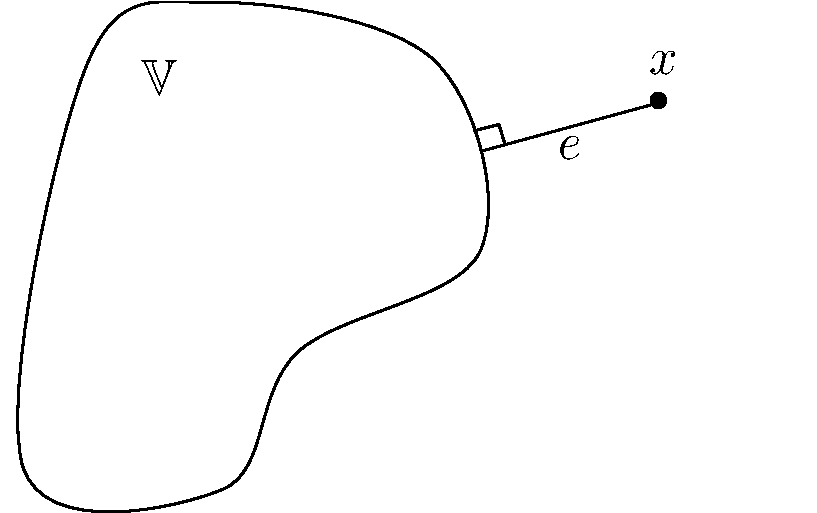
\includegraphics[width=2in]{figures/chap2_projection_on_set}
\end{center}

This is given by the orthogonal projection of $x$ onto $\mathbb{V}$.  i.e. $\iprod{ e,v} = 0 \qquad \forall v \in \mathbb{V}$

\end{frame}

%----------------------------------
\begin{frame}\frametitle{Applications to Engineering}
Let $\nbf$ be a unit vector in $\mathbb{R}^3$ (i.e., $\norm{\nbf}=1$), then 
\[
\Pi_\nbf^\perp \defeq \nbf \nbf^\top
\]
is a projection operation.  Geometrically $\Pi_\nbf^\perp x = \nbf \nbf^\top x$ find the projection of $x$ along the unit vector $\nbf$

Also 
\[
\Pi_\nbf = I-\nbf\nbf^\top
\]
is a projection operator.  Geometrically, $\Pi_\nbf x$ projections $x$ onto the 2D space that is orthogonal to $\nbf$.

\end{frame}

%----------------------------------
\begin{frame}\frametitle{The Projection Theorem}
\begin{theorem}
Let $\mathbb{S}$ be a Hilbert space and let $\mathbb{V}$ be a closed subspace of $\mathbb{S}$.  For any $x \in \mathbb{S}$ there exists a unique $v_0 \in \mathbb{V}$ closest to $x$;  i.e. $\norm{ x - v_0 } \leq \norm{ x - v } \quad \forall v \in \mathbb{V}$.\\


\vspace{1cm}

Furthermore $v_0$ minimizes $\norm{ x - v_0 }$ iff $x - v_0$ is orthogonal to $\mathbb{V}$.	
\end{theorem}
	
\end{frame}

%----------------------------------
\begin{frame}\frametitle{The Projection Theorem, proof}

{\bf Step 1.  Show that $v_0$ exists.}

Assume $x \notin \mathbb{V}$ and let $\delta = \inf_{v \in \mathbb{V}} \norm{ x - v } $
We need to show that in fact $\exists v_0 \in \mathbb{V}$ such that $\norm{ x - v_0 } = \delta$\\

Let $\{v_i\}$ be a sequence in $\mathbb{V}$ such that $\norm{ x - v_i } \to \delta $ and show that $\{ v_i \}$ is Cauchy.

\vfill
Need parallelogram law:
\[ 
\norm{ x + y }^2 + \norm{ x - y }^2 = 2\norm{ x }^2 + 2\norm{ y }^2.
\]
\vfill

Consider
\begin{multline*}
\norm{ (v_j - x) + (x - v_i) }^2 + \norm{ (v_j - x) - (x-v_i) }^2 \\
	= 2\norm{ (v_j-x) }^2 + 2\norm{ x - v_i }^2
\end{multline*}
\[ 
\Rightarrow \norm{ v_j - v_i }^2 = 2\norm{ v_j - x }^2 + 2\norm{ x - v_i }^2 - 4\norm{ \frac{(v_j + v_i)}{2} - x }^2
\]

\end{frame}

%----------------------------------
\begin{frame}\frametitle{The Projection Theorem, proof}
$v_i,v_j \in \mathbb{V} \quad \Rightarrow\quad \frac{v_j+v_i}{2} \in \mathbb{V} \quad\Rightarrow\quad\norm{ \frac{(v_j-v_i)}{2} - x }^2 \geq \delta^2$

\[ \Rightarrow \norm{ v_j - v_i }^2 \leq 2\norm{ v_j - x }^2 + 2\norm{ v_i - x }^2 - 4\delta^2 \]
But $\norm{ v_j - x } \to \delta$
\[ \Rightarrow \norm{ v_j - v_i } \to 0 \] and is therefore Cauchy.

\vfill

Since $\mathbb{V}$ is a Hilbert space
\[ v_i \to v_0 \in \mathbb{V}. \]

\vfill

Note that this proof is not constructive, i.e. it doesn't tell you how to construct the sequence $\{v_i\}$.
\end{frame}

%----------------------------------
\begin{frame}\frametitle{The Projection Theorem, proof}
{\bf Step 2.  Show that $v_0 = \arg\min_{v\in\mathbb{V}} \norm{ x - v } \Rightarrow x - v_0 \perp \mathbb{V}$}.

Proof by contradiction. Suppose that $x-v_0$ is not perpendicular to $\mathbb{V}$.  Then there exists a $v \in \mathbb{V}$ such that 
\[ \iprod{ x - v_0, v} = \delta \neq 0 \]
and w.l.o.g. (why?) let $\norm{ v } = 1$

\vfill

Let $z = v_0 + \delta v \in \mathbb{V}$ then 
\begin{flalign*}
\norm{ x - z }^2 = \norm{ x - v_0 - \delta v }^2 &= \norm{ x - v_0 }^2 - 2 Re \iprod{ x - v_0, \delta v} + \norm{ \delta v }^2 \\
&= \norm{ x - v_0 }^2 - 2 \delta^2 + \delta^2 < \norm{ x - v_0 }^2
\end{flalign*}
which is a contradiction since $v_0$ is the minimizer.
\end{frame}


%----------------------------------
\begin{frame}\frametitle{The Projection Theorem, proof}

{\bf Step 3.}
Suppose $(x - v_0) \perp \mathbb{V}$ then $\forall v \in \mathbb{V}$ such that $v \neq v_0$
\begin{align*}
\norm{ x - v }^2 &= \norm{ x - v_0 + v_0 - v }^2\\
&= \norm{ x - v_0}^2 + 2 Re \iprod{ x - v_0, v_0 - v} + \norm{ v_0 - v }^2\\
&= \norm{ x - v_0 }^2 + \norm{ v_0 - v }^2\\
&> \norm{ x - v_0 }^2
\end{align*}

{\bf Step 4. Uniqueness}
Same as proof on page 25 of notes.
	
\end{frame}

%----------------------------------
\begin{frame}\frametitle{Closed Subspace}
\begin{theorem}[Moon Theorem 2.10]
Let $\mathbb{V}$ be a closed subspace of a Hilbert space $\mathbb{S}$, then
\begin{flalign*}
\mathbb{S} &= \mathbb{V} \oplus \mathbb{V}^{\perp}\\
\mathbb{V} &= \mathbb{V}^{\perp \perp}
\end{flalign*}
\end{theorem}
\begin{proof}
In book.	
\end{proof}
	
\end{frame}



\end{document}